\documentclass[8pt]{beamer}

\usepackage[utf8]{inputenc}
\usepackage{eurosym}
\RequirePackage[francais]{babel}
%\usepackage{url}
%\usepackage{etex}
%\usepackage{enumitem}
%\usepackage{multicol}
\usepackage{xcolor}
%\usepackage{bbm}
%\usepackage{amsmath,amsthm,amssymb}
%\usepackage[official]{eurosym}
%\usepackage{pifont}
%\usepackage{exercise}
%\usepackage{graphics}
%\usepackage{array,multirow,makecell}
\usepackage{verbatim}
%\usepackage[dvipsnames]{pstricks}
\usepackage{pstricks-add,pst-plot,pst-text,pst-tree,pst-eps,pst-fill,pst-node,pst-math,pst-blur,pst-func}
%\usepackage{pgf,tikz}
%\usepackage{tipfr}
%\usepackage{thmbox}
%\usepackage{calc}
%\usepackage{ifthen}
%\usepackage{pdfpages}
%\usepackage{colortbl}
%\usepackage{sagetex}
%\usetikzlibrary{arrows,patterns}
%\input tabvar
%\usepackage{tkz-tab}
%\usepackage{listings}
%\usepackage[np]{numprint}
%\usepackage{fancybox,fancyhdr}
%\usepackage{thmtools}
%\usepackage{bclogo}
%\usepackage{lastpage}

\usepackage{tabularx}
\usepackage{array,multirow,makecell}
\usetheme{Madrid}
%\usetheme{Bergen}
\usecolortheme{beaver}
 
%Information to be included in the title page:
\title{Requête HTTP}
\subtitle{Méthodes GET et POST}
\author{Yannick CHISTEL}
\institute{Lycée Dumont d'Urville - CAEN}
\date{\today}
 
%----------------------------------------------------------------------------------------------- 
% 							Commandes Tableaux
%-----------------------------------------------------------------------------------------------
\setcellgapes{1pt}
\makegapedcells
\newcolumntype{R}[1]{>{\raggedleft\arraybackslash }b{#1}}
\newcolumntype{L}[1]{>{\raggedright\arraybackslash }b{#1}}
\newcolumntype{C}[1]{>{\centering\arraybackslash }b{#1}}

\definecolor{vert}{rgb}{0,0,1}


\newcounter{num}
\setcounter{num}{0}
 
\begin{document}
 
\frame{\titlepage}

\begin{frame}
\frametitle{Requête HTTP}

\begin{block}{Introduction}
%On accède aux éléments d'un tableau avec leurs indices.

HTTP est un protocole qui permet de récupérer des ressources comme les documents HTML, des images ou autres médias. Il est à la base de tout échange de données sur le Web. C'est un protocole de type client-serveur.

\begin{center}
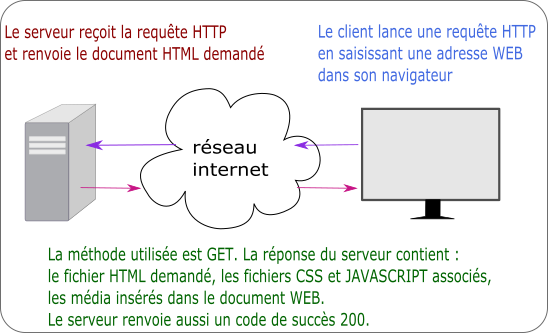
\includegraphics[scale=0.66]{img/requeteHTTP.eps}
\end{center}
\end{block}

\end{frame}


\begin{frame}
\frametitle{Les méthodes de requête HTTP}

\begin{block}{Méthodes}
Une requête HTTP possède plusieurs méthodes:
\begin{enumerate}
\item La methode \textbf{GET} qui récupère du serveur les données HTML du document demandé;
\item La méthode \textbf{POST} qui envoie au serveur des données (formulaire);
\item La méthode \textbf{DELETE} qui supprime des données sur le serveur.
\end{enumerate}

Le serveur répond à la requête selon la méthode utilisée. Sa réponse contient un code d'état. Les codes d'état sont classés par catégorie. Les plus courants sont :
\begin{enumerate}
\item Si la requête est un succès, le code d'état vaut 200;
\item Si la requête a été redirigée vers un autre site web, le code d'état vaut 301;
\item Si la ressource n'est pas accessible, accès refusé, le code d'état vaut 403;
\item Si la ressource demandée n'est pas trouvée, le code vaut 404;
\item Si le serveur ne peut pas répondre (panne), le code vaut 500;
\end{enumerate} 


\end{block}
\end{frame}




\begin{frame}
\frametitle{Exemple de requête HTTP avec la méthode GET}

\begin{exampleblock}{Exemple}
Dans un navigateur, on saisit une url :
\begin{center}

\includegraphics[scale=0.7]{img/url-site.eps}
\end{center}
Le navigateur envoie la requête au serveur qui héberge la page WEB demandée. L'en-tête d'envoi contient de nombreuses informations dont :
\begin{itemize}
\item La méthode utilisée est \textbf{GET} et la version du protocole est \textbf{HTTP/1.1};
\item La ressource demandée est une image d'extension \textbf{jpg};
\item Le serveur (domaine) interrogé est \textbf{interstices.info};
\item Le client HTTP utilisé est le navigateur de \textbf{Mozilla} c'est à dire \textbf{FIREFOX} version \textbf{86} dans un environnement \textbf{WINDOWS};
\item Tous les formats d'images sont acceptés \textbf{*/*} et aussi compressés \textbf{webp};
\item La langue acceptée est le français et aussi l'anglais.
\end{itemize}
\begin{center}
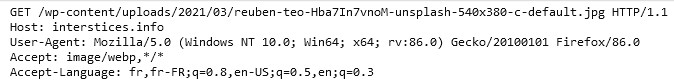
\includegraphics[scale=0.65]{img/requete-img.eps}
\end{center}

\end{exampleblock}

\end{frame}



\begin{frame}
\frametitle{Exemple de réponse HTTP avec la méthode GET}

\begin{exampleblock}{Exemple}
Le serveur reçoit une requête avec la méthode \textbf{GET}. Il analyse la requête et répond en renvoyant la ressource demandée et l'en-tête de la réponse contient les éléments suivants:

\begin{itemize}
\item Le code d'état de la réponse est \textbf{200} ce qui signifie que la ressource demandée a été trouvée et envoyée au client \textbf{OK};
\item La date et l'heure de l'envoi;
\item Le serveur utilise l'application \textbf{Apache} (serveur web);
\item Le type de la ressource envoyée est une image \textbf{jpeg} et la taille est $63058$ octets.
\item La connexion est fermée après la réponse. 
\end{itemize}
\begin{center}
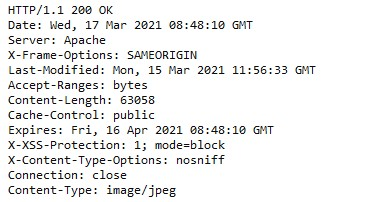
\includegraphics[scale=0.7]{img/reponse-img.eps}
\end{center}

\end{exampleblock}

\end{frame}


%\begin{frame}
%\frametitle{Fichiers récupérés par des requêtes HTTP avec la méthode GET}
%
%\begin{exampleblock}{Exemple}
%\begin{center}
%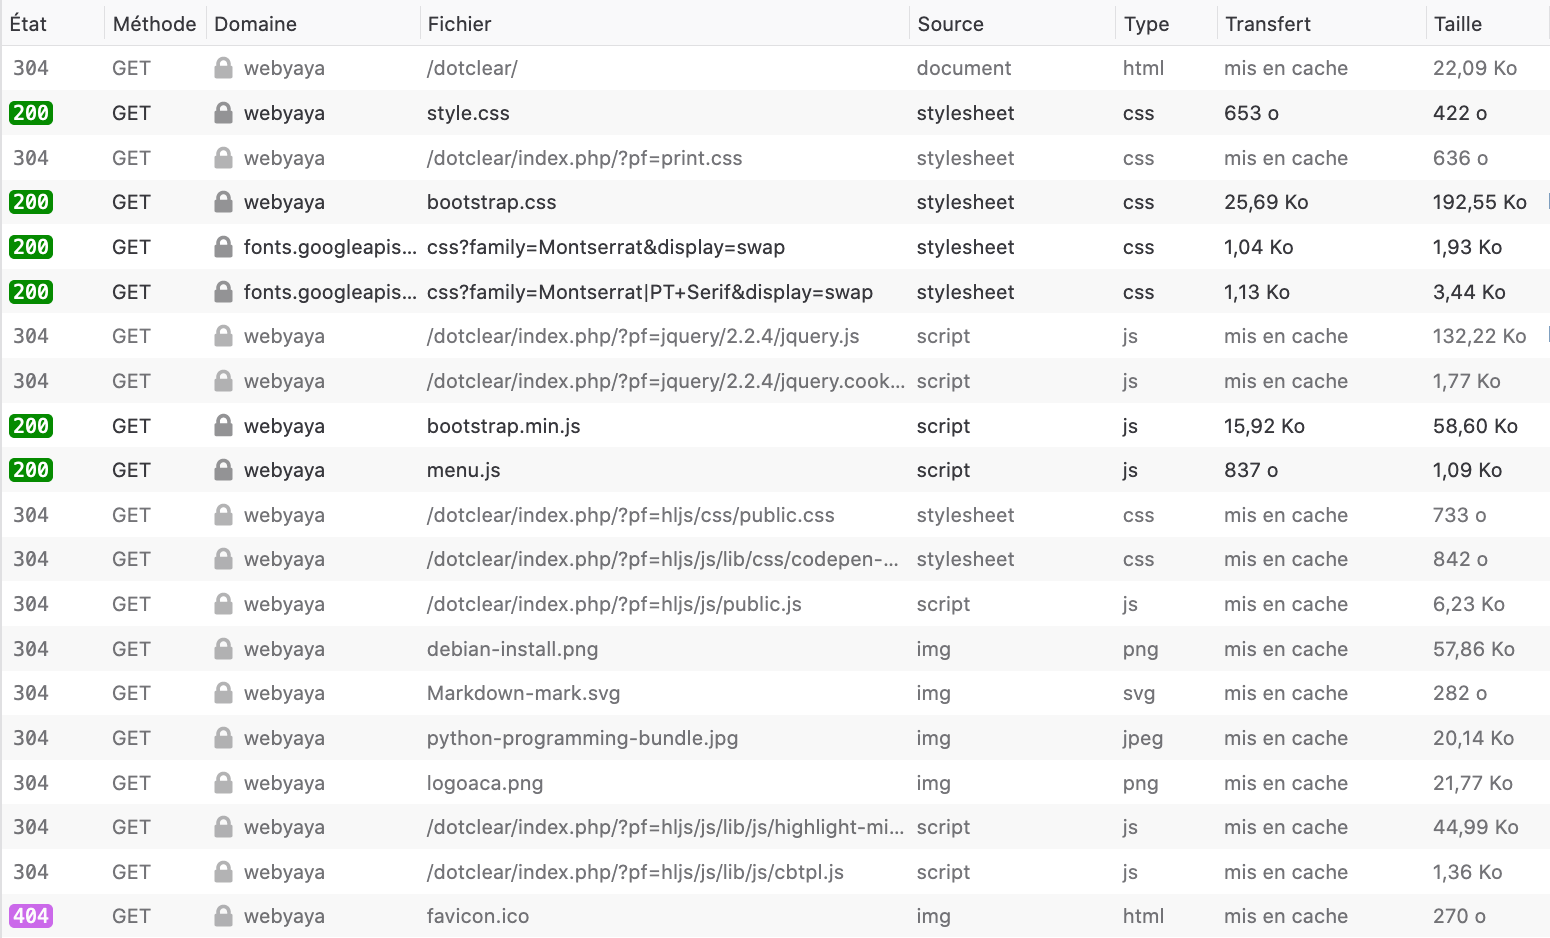
\includegraphics[scale=0.42]{img/requeteHTTP-getfichiers.eps}
%\end{center}
%
%\end{exampleblock}
%
%\end{frame}

\begin{frame}
\frametitle{Requête HTTP et paramètres}

\begin{block}{Méthode GET}
La méthode GET permet d'envoyer des paramètres au serveur qui les analysera et adaptera sa réponse aux valeurs des paramètres. 
La syntaxe utilise :
\begin{itemize}
\item le \textbf{point d'interrogation (?)} pour séparer l'url des paramètres;
\item les paramètres et les valeurs reliés par le signe \textbf{égal (=)};
\item les différents paramètres sont séparés par des \textbf{esperluettes (\&)}.
\end{itemize}
\end{block}

\begin{exampleblock}{Exemple}
\begin{center}
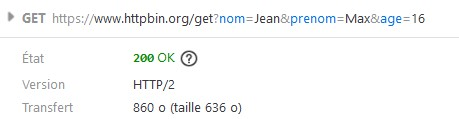
\includegraphics[scale=0.6]{img/get-param.eps}
\end{center}
\end{exampleblock}

\begin{alertblock}{Remarque}
\begin{enumerate}
\item Le passage de valeurs par l'url est surtout employé pour rediriger le client vers des ressources particulières selon les contenus : \textbf{article}, \textbf{rubrique}, \textbf{media} etc.
\item Cette méthode est à proscrire pour l'envoi de données secrètes comme un mot de passe !
\end{enumerate}
\end{alertblock}
\end{frame}


\begin{frame}
\frametitle{Requête HTTP et paramètres}

\begin{block}{Méthode POST}
La méthode POST permet d'envoyer des paramètres au serveur. Les paramètres et les valeurs sont placés dans le \textbf{corps de la requête} soit:
\begin{enumerate}
\item sous la forme d'une chaine de caractères (comme pour la méthode GET)
\item sous la forme de donnée structurée qui est dans la majorité des cas le \textbf{JSON}. 
\end{enumerate}

L'usage d'un formulaire dans la page web est alors employé pour présenter les différents paramètres et les zones de saisie permettent d'y associer les valeurs. Un bouton d'envoi permet l'envoi des données.
\end{block}

\begin{block}{Réponse à une requête POST}
Les données d'une requête POST sont analysées par le serveur et plus précisément par un script qui va construire une réponse:
\begin{enumerate}
\item soit sous la forme d'une structure de donnée de type JSON et un script (javascript) sur le client mettra à jour la page web.
\item soit sous la forme d'une nouvelle page web (HTML) qui sera affichée par le navigateur.
\end{enumerate}

Les requêtes HTTP avec la méthode POST nécessitent un traitement des données et l'envoi d'une réponse vers le client. On parle dans ce cas de page web dynamique.
\end{block}
\end{frame}


\begin{frame}
\frametitle{Exemple de requête HTTP avec la méthode POST}

\begin{exampleblock}{Exemple}
\begin{center}
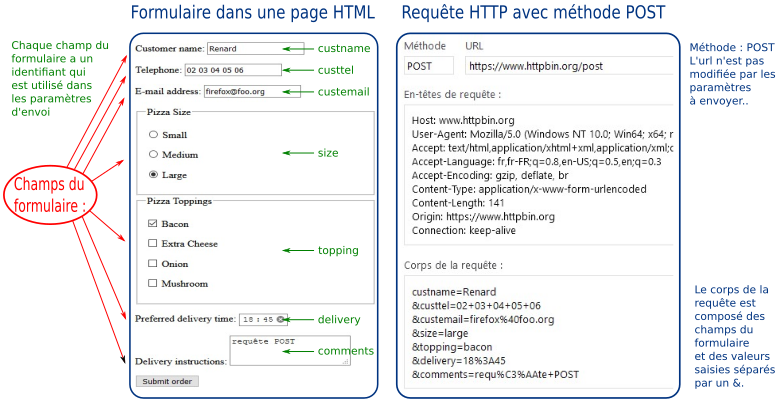
\includegraphics[scale=0.58]{img/requete-POST.eps}
\end{center}
\end{exampleblock}

\end{frame}



\end{document}

